La réalisation de ce travail de Bachelor a nécessité une gestion rigoureuse du temps et des ressources. Pour assurer une progression régulière et structurée du projet, une méthodologie de travail spécifique a été mise en place. Cette méthodologie a été centrée autour de trois piliers principaux : la planification, le suivi du temps et la documentation.

\section{Planification}

La planification a été un pilier fondamental de la méthodologie de travail. Pour ce faire, j'ai utilisé un tableau blanc pour organiser et visualiser le projet de manière dynamique. Ce tableau, constamment mis à jour, a servi à décomposer le projet en tâches plus petites et à les organiser en sprints, qui sont des périodes de travail dédiées à la réalisation d'un ensemble spécifique de tâches.

En général, en début de semaine, je prenais un moment pour définir et prioriser les tâches à accomplir pendant le sprint sur le tableau blanc. Cette méthode visuelle et interactive m'a permis de garder une vue d'ensemble du projet et de suivre son avancement en temps réel. De plus, elle m'a offert la flexibilité nécessaire pour ajuster la planification en fonction de l'évolution du projet.

\begin{figure}[H]
    \centering
    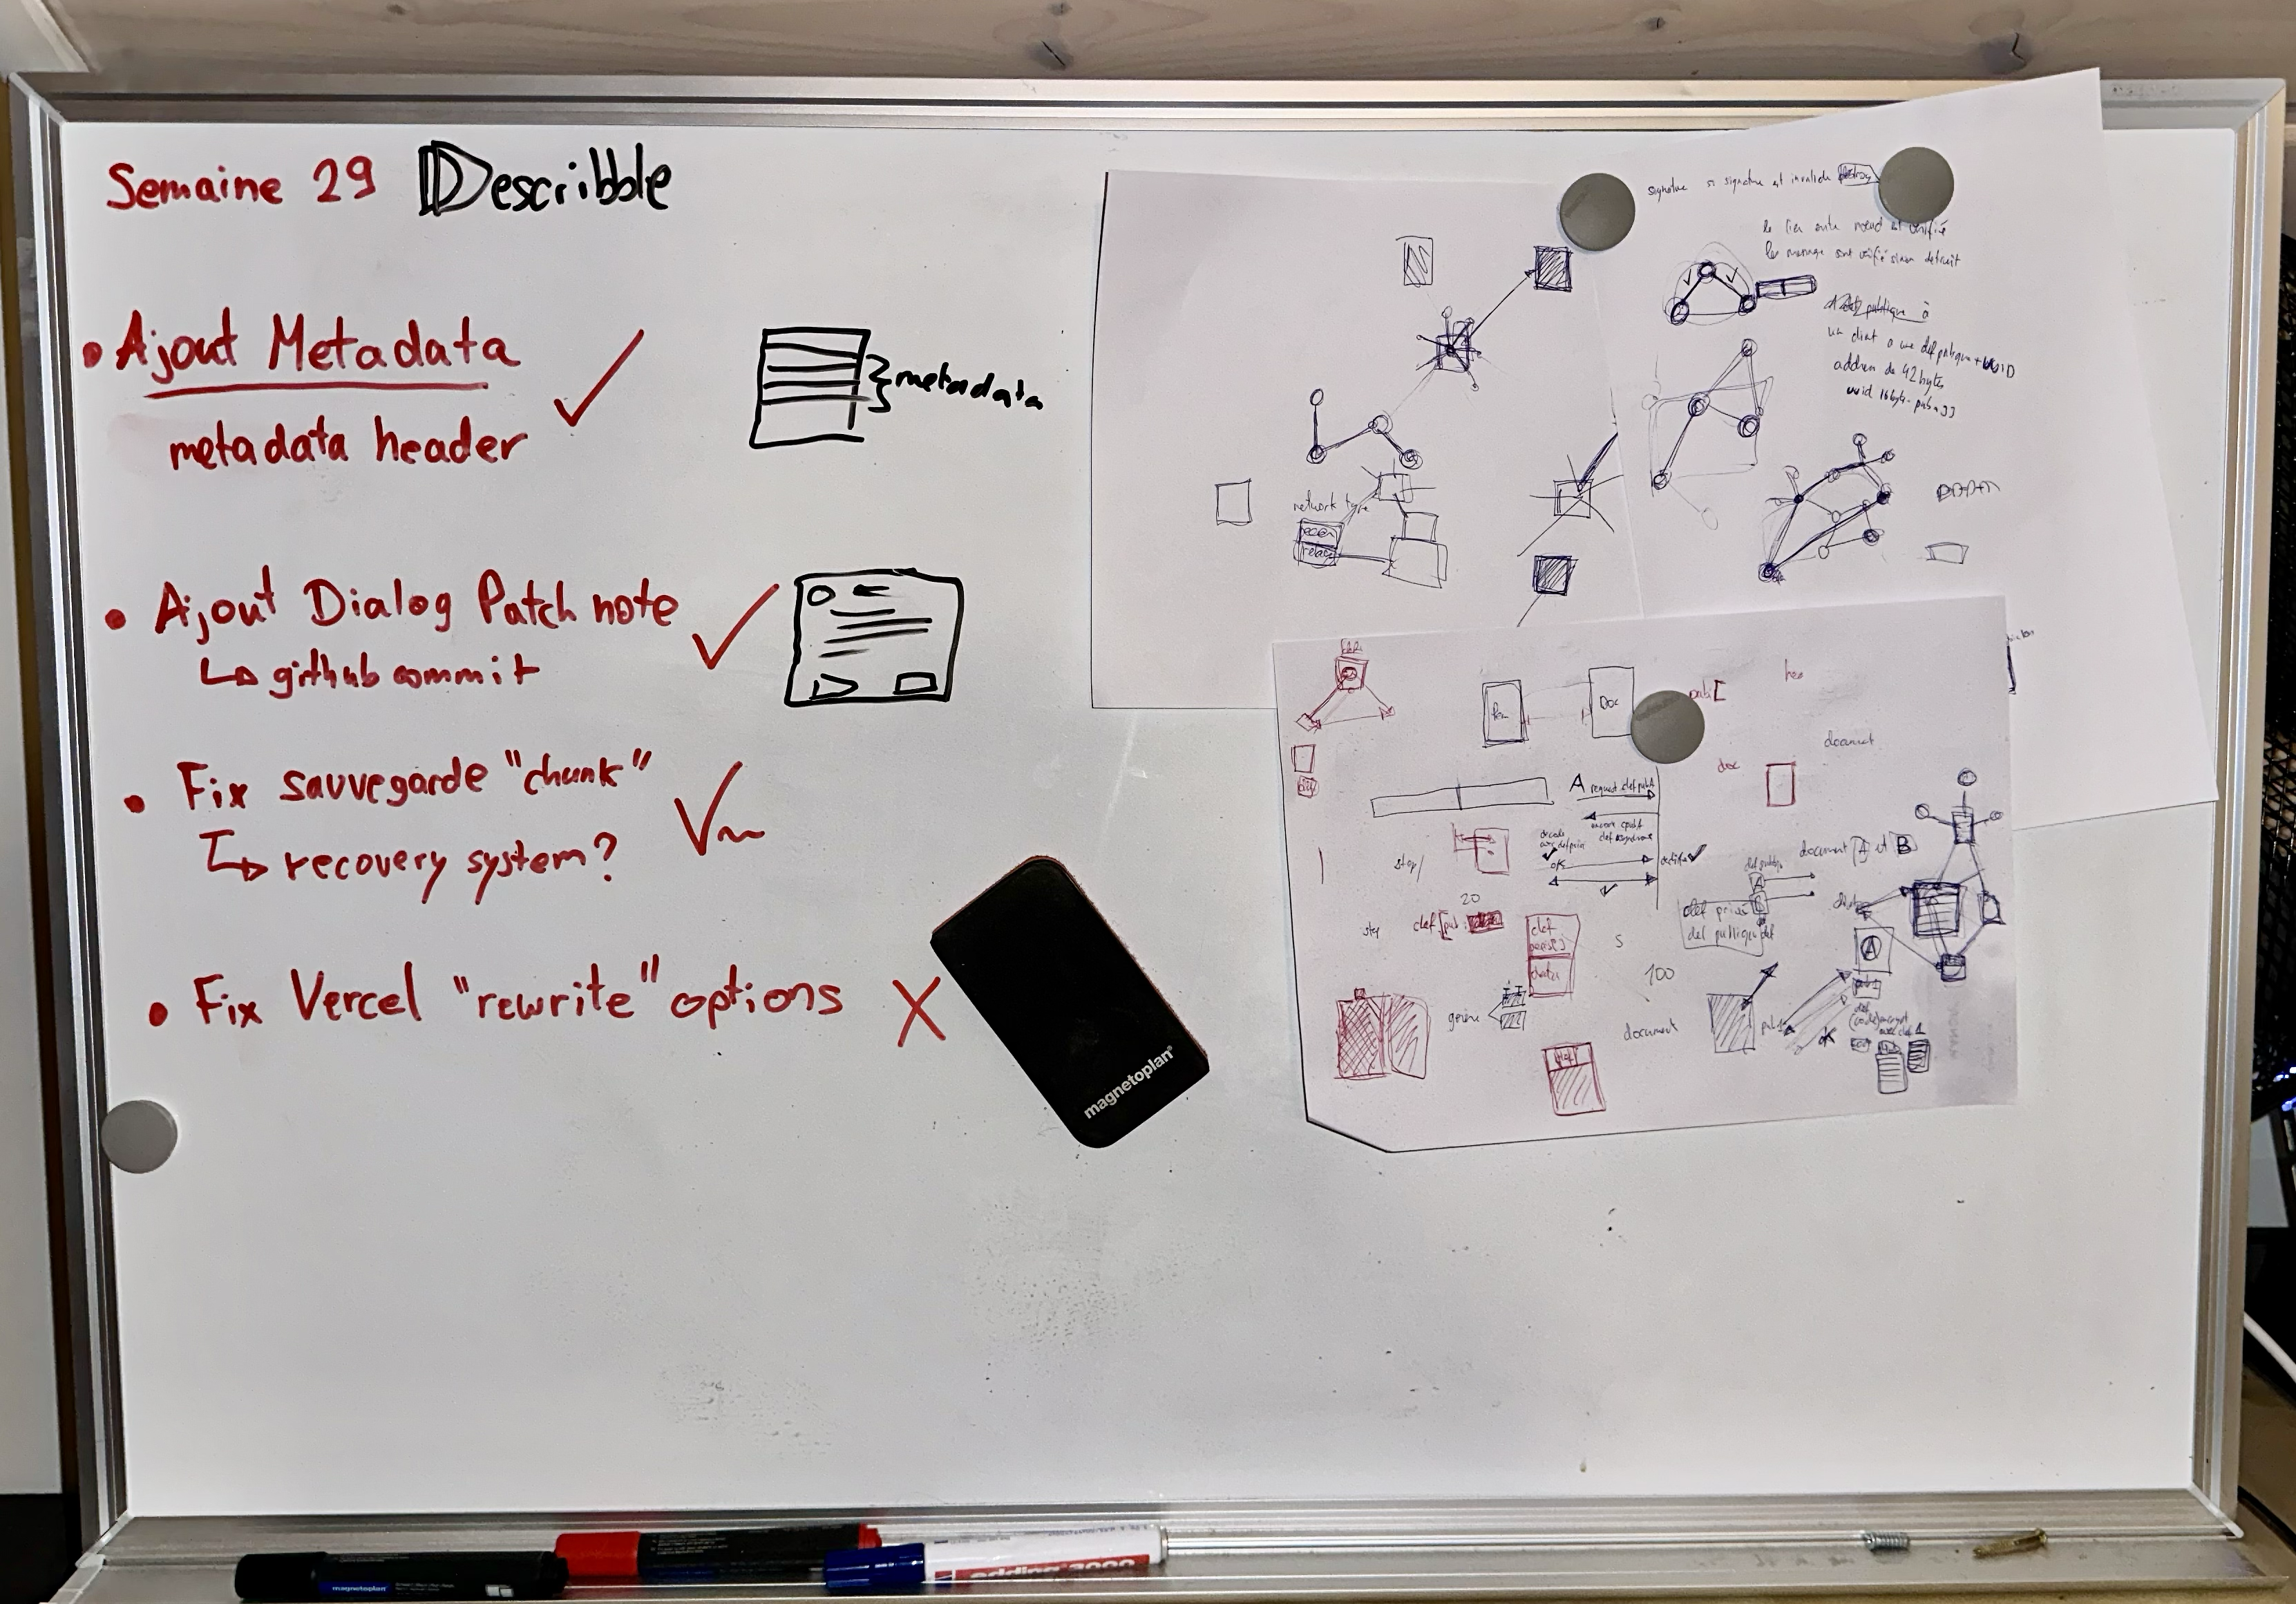
\includegraphics[width=0.9\textwidth]{assets/figures/planning.png}
    \caption{Exemple de planification sur un tableau blanc}
\end{figure}

\section{Suivi du temps}

Le suivi précis du temps passé sur chaque tâche est un aspect crucial de la gestion de projet. Pour ce faire, l'outil Wakatime a été utilisé. Wakatime est un outil de suivi du temps dédié aux développeurs. Il offre une variété de statistiques relatives au temps passé à coder, telles que le temps passé par jour, par semaine, par mois, ou encore le temps passé sur chaque fichier ou projet.

Ces statistiques ont permis de garder une trace précise du temps investi dans le projet, mais ont aussi servi à ajuster la répartition du temps en fonction des besoins identifiés. Par exemple, si une tâche s'avérait plus longue que prévu, le planning pouvait être réajusté en conséquence.

\begin{figure}[H]
    \centering
    \includegraphics[width=0.9\textwidth]{assets/figures/wakatime.png}
    \caption{Exemple de statistiques fournies par Wakatime}
\end{figure}

\section{Documentation}

La documentation a été un autre aspect essentiel de la méthodologie de travail. Chaque portion de code produite a été soigneusement documentée. Cela avait pour but de faciliter la compréhension du projet pour quiconque souhaitait le comprendre ou y contribuer à l'avenir.

En plus de documenter le code, le projet a été publié sous forme de packages sur le gestionnaire de paquets Node.js (npm). Ces packages ont été soigneusement documentés pour permettre à d'autres développeurs de comprendre leur fonctionnement et de les utiliser dans leurs propres projets. La documentation des packages npm est particulièrement importante car elle fournit aux développeurs des informations cruciales sur la manière d'installer et d'utiliser les packages.

Le dépôt GitHub du projet a également été maintenu dans un état propre et bien organisé. Cela a permis de faciliter la navigation à travers le projet et d'améliorer sa maintenabilité.

\begin{figure}[H]
    \centering
    \includegraphics[width=0.9\textwidth]{assets/figures/npm-package.png}
    \caption{Exemple de package publié sur npm avec une documentation détaillée. Le package peut être trouvé à l'adresse suivante: \url{https://www.npmjs.com/package/@describble/ddnet}}
\end{figure}

Cette approche méthodologique, alliant une planification rigoureuse, un suivi précis du temps de travail et une documentation approfondie, a été essentielle pour mener à bien le projet de manière structurée et efficace. Elle a également grandement contribué à la qualité du travail final.